\documentclass[a4paper,11pt]{article}
\usepackage{CLARIN2015}
\usepackage[english]{babel}
%\usepackage{hyperref}{}

\usepackage{times}  
\usepackage{url}
\usepackage{graphicx}



\pagestyle{empty}
\begin{document}



\title{FoLiA in practice: The infrastructure of a linguistic annotation format}
\author{Maarten van Gompel$^a$ \and Ko van der
    Sloot$^a$ \and Martin Reynaert$^{ab}$ \and Antal van den Bosch$^c$} %cheating to get the affiliation footnotes right
\date{}


\maketitle
\renewcommand{\thefootnote}{\alph{footnote}}
\footnotetext[1]{Centre for Language and Speech Technology, Radboud University}
\footnotetext[2]{Tilburg Centre for Cognition and Communication, Tilburg University}
\footnotetext[3]{Centre for Language Studies, Radboud University}
\renewcommand{\thefootnote}{\arabic{footnote}}

\begin{abstract}
We present an overview of the software and data infrastructure around FoLiA, a
\textbf{Fo}rmat for \textbf{Li}nguistic \textbf{A}nnotation developed in the
scope of the CLARIN-NL project and other projects.  FoLiA aims to provide a
single unified file format accommodating a wide variety of linguistic
annotation types, preventing the proliferation of using different formats for
different annotation types. FoLiA is being developed in a bottom-up and
practice-driven fashion.  We have invested mainly in the creation of a rich
infrastructure of tools that enable developers and end-users to work with the
format. This work will present the current state of this infrastructure.
\end{abstract}


\section{Introduction}

CLARIN's aim is to deliver an infrastructure for researchers that work with
language data and tools. This is impossible without agreeing on standards with
regard to data formats. Standardisation is an important prerequisite for good
interoperability between the many language tools that have emerged within and
outside of the scope of the CLARIN project, and to ensure the various data sets
released are usable in practice.

In the field, however, we often encounter an abundance of ad-hoc formats. We
define ad-hoc formats to be data formats that are characterised by most of the
following traits:

\begin{itemize}
    \item They are only used once, often by one specific tool or for just one specific purpose;
    \item They are poorly formalised or not formalised at all, i.e. there is a lack of a formal schema and semantics;
    \item They are poorly documented;
    \item They are often rigid and hard to extend.
\end{itemize}

The use of such ad-hoc formats can be considered the opposite of proper
standardisation and is to be avoided in any large infrastructure project.

CLARIN adheres to the following principles when it comes to standardisation:

\begin{itemize}
    \item Open standards are preferred over proprietary standards;
    \item Formats and protocols should be:
    \begin{itemize}
        \item well-documented
        \item verifiable
        \item proven (being used in practice);
    \end{itemize}
    \item Text-based formats are (where possible) preferred over binary formats.
\end{itemize}

Fortunately, there are various initiatives for standardisation resulting in
annotation formats that transcend the ad-hoc level, each with their own merit, and ours
being of one of them. At the onset of CLARIN-NL, however, the Dutch and Flemish
Natural Language Processing (NLP) community lacked such a proper standard with
respect to linguistically annotated text, and ad-hoc formats were prevalent in
the field.  In the scope of CLARIN-NL project TTNWW, the NWO project
DutchSemCor, and the STEVIN project SoNaR, FoLiA (Format for Linguistic
Annotation) was developed as a solution to accommodate their representational
needs.

The aim of FoLiA is to provide a practical standard, following a generic
paradigm, for the linguistic annotation of primarily written text. For this purpose,
a wide variety of linguistic annotation types is supported. 

In this current paper, we intend to focus on the \emph{practical} nature of the
format, or rather, on the infrastructure that is built around the format,
software that supports it, and the ways in which it has been put to use in the
scope of CLARIN and beyond.  Section~\ref{sec:philosophy} will explain our
philosophy behind FoLiA and its infrastructure. 

An extensive overview of the format has already been presented in earlier work
\cite{FOLIACLIN2013}. This aforementioned work also addresses the motivation
for the creation of FoLiA and presents a comparison with similar initiatives
such as the D-Spin Text Corpus Format (TCF), PAULA XML, XCES, as well as with
more abstract frameworks such as LAF (Linguistic Annotation Format) and
comprehensive text-encoding formats such as TEI. We recognize that FoLiA is
just one out of various possible solutions, and claim its merit is best decided
on its practical usability with respect to the user's specific purpose. The
tools, libraries and existing FoLiA-delivered corpora described in the current work
are intended to help people assess whether FoLiA is an appropriate solution for
their tasks.

Full documentation of FoLiA is available elsewhere \cite{FOLIADOC2014}. It
offers a reference guide to all elements and attributes that FoLiA defines.  A
brief summary of key features will be repeated in Section~\ref{sec:overview}.
Section~\ref{sec:softwareinfrastructure} subsequently presents the currently
available software infrastructure for FoLiA.
Section~\ref{sec:datainfrastructure} presents some corpora that have been
delivered in FoLiA.

\section{Overview}
\label{sec:overview}

FoLiA is an XML-based format and defines specific XML elements for \emph{structure
annotation} (e.g. paragraphs, sentences, word tokens, lists, figures, etc.) and
\emph{linguistic annotation} (e.g. part-of-speech, dependency relations,
syntax, named entites, etc.). FoLiA makes use of a combination of inline and
stand-off annotation, making proper use of the hierarchical nature of XML and
facilitating the job for parsers where possible. The format is fully language and
tagset independent as tagsets are defined separately in \emph{FoLiA Set Definitions}
by users and never prescribed by FoLiA itself. Validation can proceed
on a shallow level, against a RelaxNG schema, as well as on a deep level which
validates the used tagsets against the set definition files.

The sets are at the core of the FoLiA paradigm, annotation elements take a
generic attribute named ``class''. These \emph{classes} pertain to a set and are
defined by whatever set definition the user decides to use. The set definition
defines all allowed classes and allows for links with data category registries
for formal semantic closure.

Other generic attributes besides ``class'' are attributes to denote the
annotator of a particular annotation, the annotator type (human or machine),
the confidence level of the annotation, the time of the annotation, and more.

FoLiA also allows for various types of \emph{higher-order annotation}, such as
the ability to include alternative annotations, as well as extensive support
for corrections on annotations. Moreover, there is the possibility to link other
modalities, such as audio fragments of speech, to structural elements. So, even
though FoLiA is primarily a format to annotate text documents, speech
transcripts are supported as well. 

For metadata CLARIN-NL was committed to the CMDI standard \cite{CMDI}.
Although FoLiA has simple native support for metadata, we see no
sense in reinventing the wheel and FoLiA is ideally used in combination with an
external metadata format such as CMDI whenever extensive metadata is desired. A
reference to the metadata file can be made in the header of the FoLiA document.

The FoLiA paradigm laid out here is schematically illustrated in
Figure~\ref{fig:paradigm} \cite{FOLIADOC2014}. A more in-depth treatise is beyond the scope of this
current paper.

\begin{figure}[h]
\begin{center}
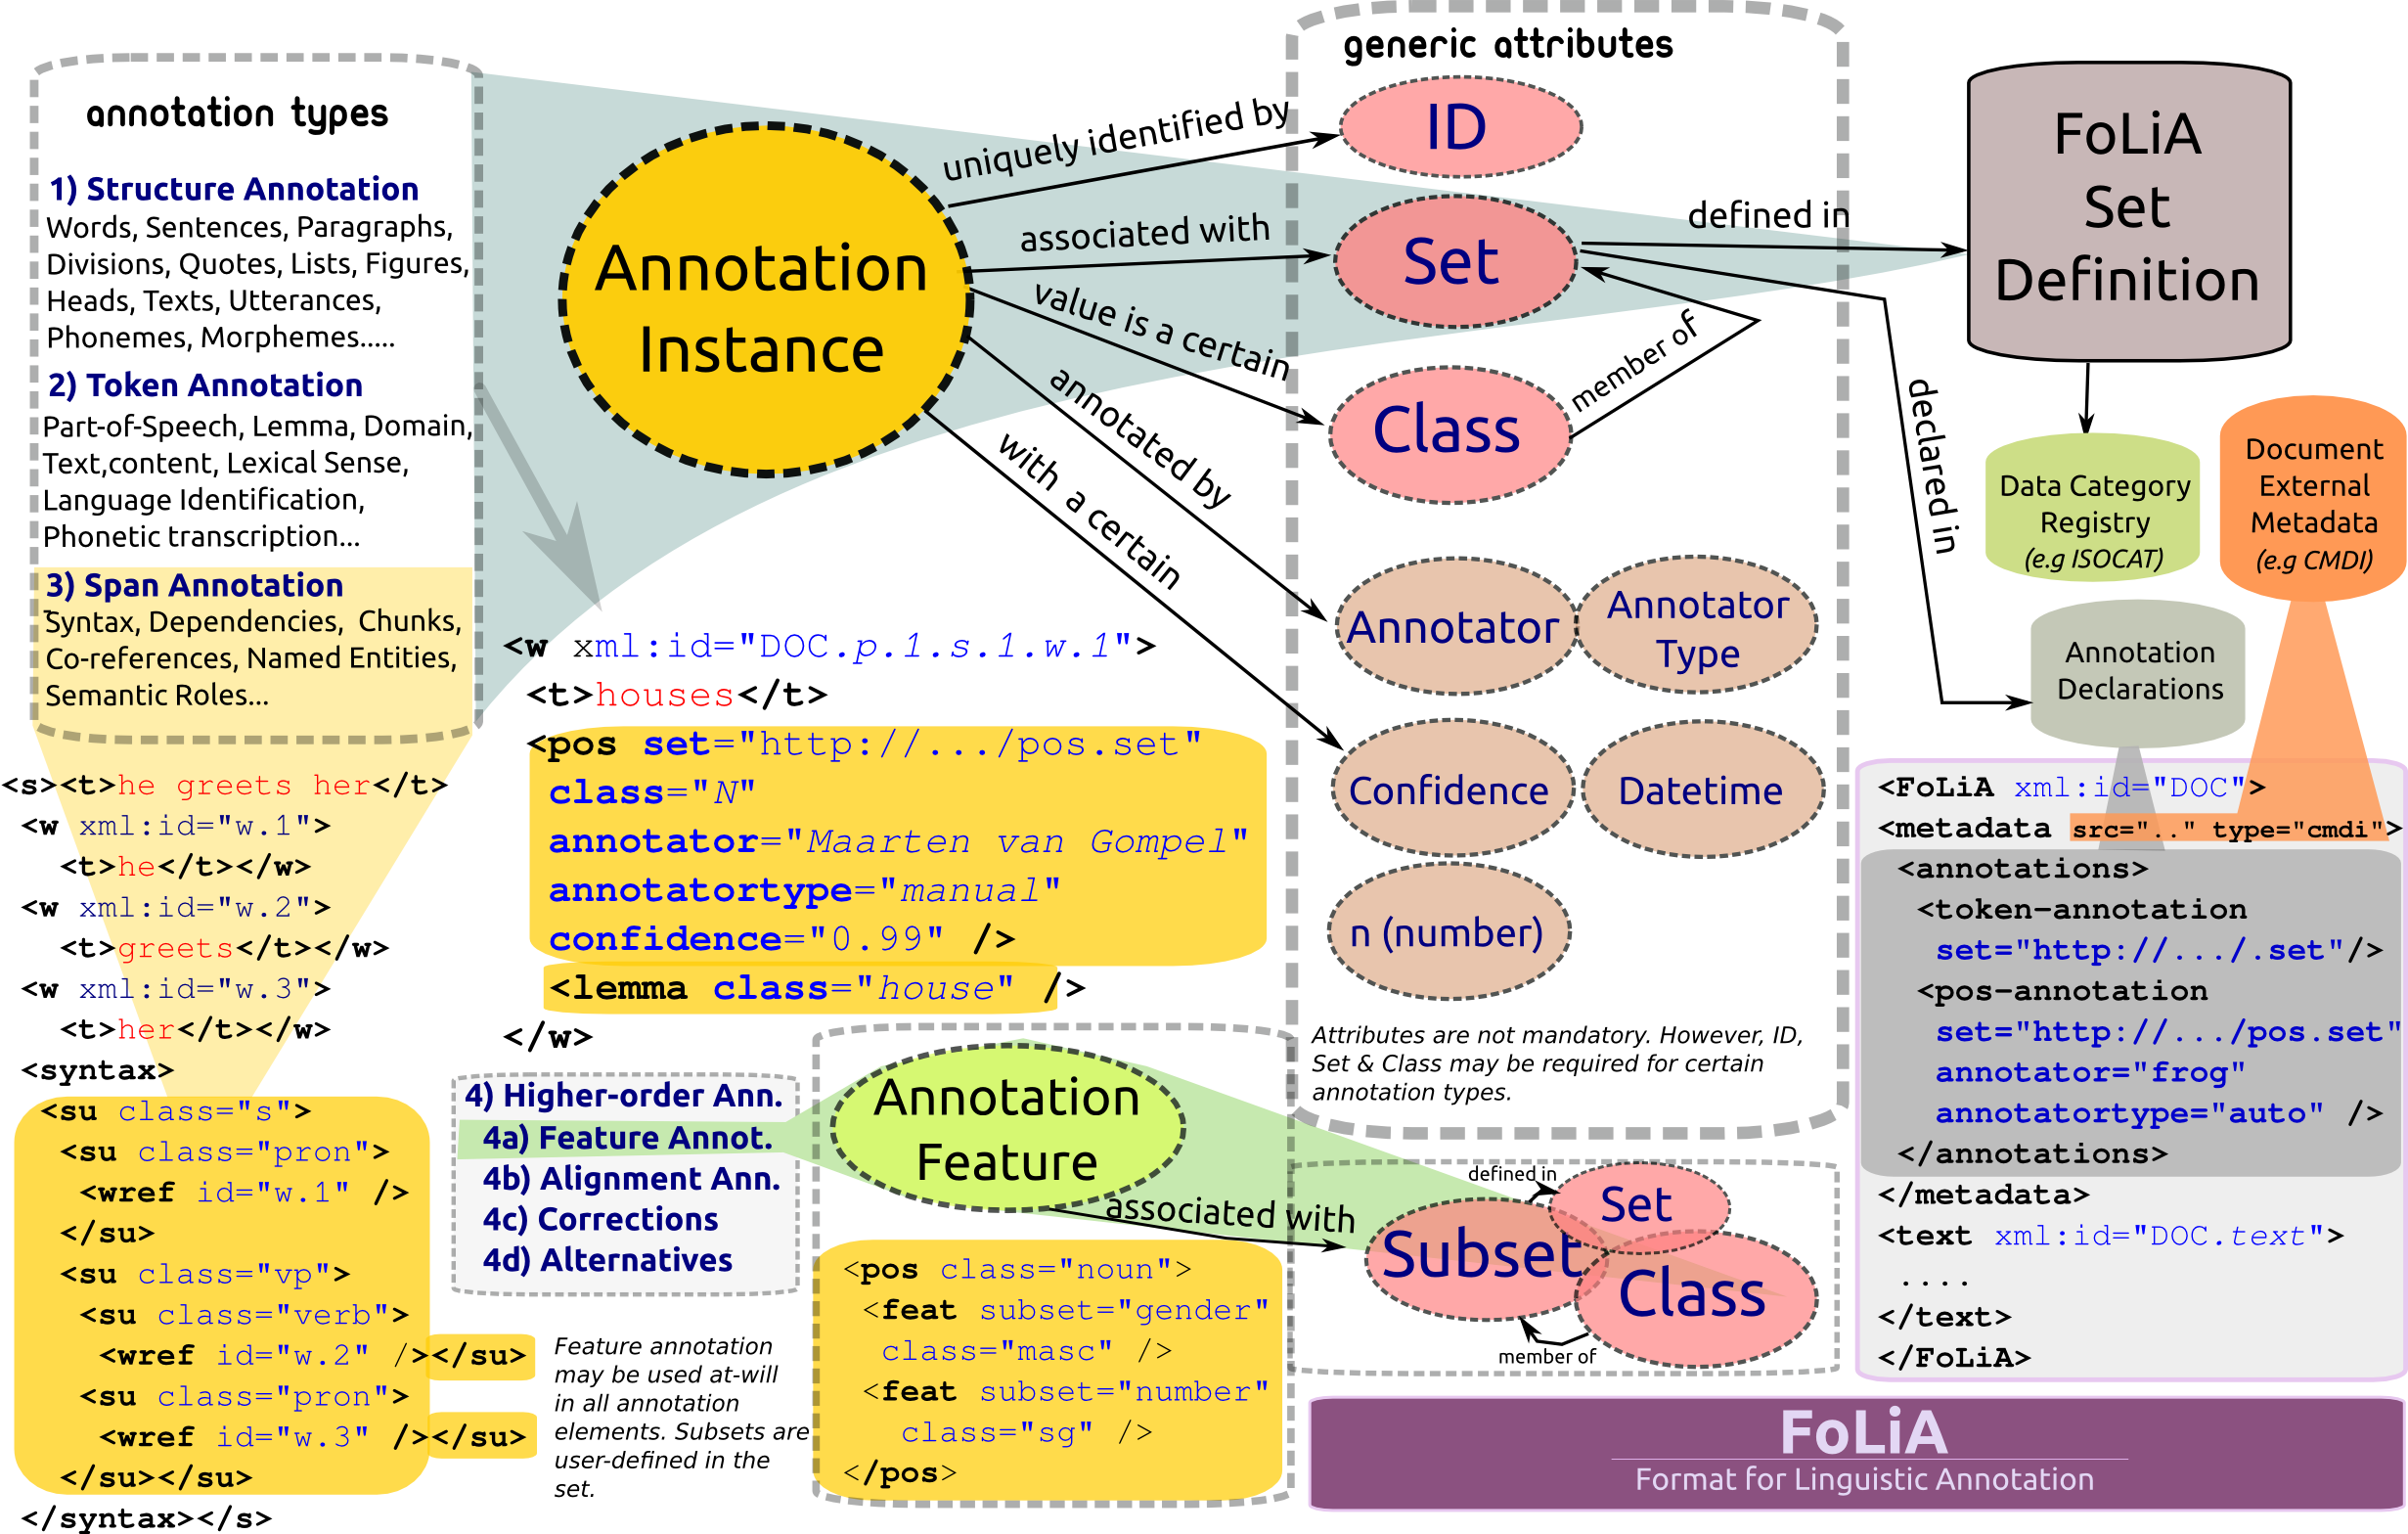
\includegraphics[width=160.0mm]{folia_paradigm.png}
\end{center}
\caption{A schematic overview of the most important aspects of the FoLiA
paradigm, including XML examples \cite{FOLIADOC2014}.}
\label{fig:paradigm} 
\end{figure}

\section{Our philosophy}
\label{sec:philosophy}

Recalling the CLARIN principle that a format should be proven and used in
practice, FoLiA has been designed in a bottom-up manner taking especially this
principle to heart. Our focus is to solve real problems people face in the
field with regards to their linguistic representation needs, and to do so in a
generic manner. The ambition is to deliver a single unified file format that
can effectively handle a multitude of annotation needs in a generic way.
The main motivation is to prevent the need to switch formats whenever an extra
annotation type is introduced, and to prevent the scenario in which a plethora
of different formats is used for different annotation types.

It is nevertheless always conceivable that a user's particular need is not yet
covered by the latest version of FoLiA; in such cases we gladly hear from the
user and expand FoLiA where necessary, in collaboration with the user. The
development of FoLiA has already proceeded for several years in such a
collaborative workflow, and various annotation types have been added in close
contact with end-users both from within CLARIN and beyond.

In our philosophy, the creation of a file format is useless without
simultaneously creating an infrastructure of tools to work with said format.
This has therefore been our main focus over the years and will be the subject
of the next section.

\section{Software Infrastructure}
\label{sec:softwareinfrastructure}

When we speak of a FoLiA software infrastructure we refer to a published set of
software, from whatever sources and for whatever architecture, that enable
people to work with FoLiA. Such an infrastructure in simple terms encompasses
anything that can either process or deliver the data in the format. We can
subdivide it into the following components:

\begin{enumerate}
\item programming libraries;
\item tools for validation;
\item tools for conversion from and to other formats;
\item tools for visualisation;
\item tools for searching/querying;
\item editing tools;
\item special-purpose tools; i.e. specialised tools that use the format but are
    not necessarily focused on it. In the case of FoLiA, this includes Natural
    Language Processing or Information Retrieval tools that use the format as
    input and/or output.
\end{enumerate}

The programming libraries and tools that are purely designed to visualise,
manipulate, or convert the format in basic ways can be considered part of a
\emph{core layer} of the infrastructure, whereas the special-purpose tools can
be considered to constitute an outer layer.

As FoLiA is an XML-based format, the rich and well-established XML
infrastructure is open to its users as well. In fact, almost all FoLiA tools
effectively rely on the existing software infrastructure available for XML. 

It is possible to not use any of the FoLiA-specific tools and use the
infrastructure offered by XML directly. For instance, one can use XPath to
query a FoLiA document and XSL to transform it. To do so effectively, however,
the user/developer needs to be more familiar with the intricacies of FoLiA than when using a tool from the FoLiA infrastructure that abstracts over this
for the benefit of the user/developer.

Many of the tools of the core layer are available as command-line tools and are
bundled in two software packages: there is a Python-based \textbf{FoLiA Tools}
package\footnote{\url{https://pypi.python.org/pypi/FoLiA-tools}} and a \textbf{FoLiA
Utilities} package\footnote{\url{https://github.com/LanguageMachines/foliautils}}
consisting of tools written in C++. Both are built on the respective libraries.
There is some overlap in tools, but each also offers distinct tools the other
does not. It is therefore recommended to install both.

These packages, and all other tools pertaining to the FoLiA infrastructure
which have been developed at Radboud University, are bundled in our
\textbf{LaMachine}
distribution.\footnote{\url{https://proycon.github.io/LaMachine/}} LaMachine
greatly facilitates installation of this software and is a recommended starting
point if you work with FoLiA. It is available as a Virtual Machine, a Docker
package or a local compilation \& installation script.

We subscribe strongly to the CLARIN principle that standards should be open and
place a similar requirement on the infrastructure components we build. 

\subsection{Programming Libraries}

At the heart of the FoLiA infrastructure are the \emph{programming libraries} that
enable developers to work with documents in the format in their software. We
ourselves offer libraries for both Python and for C++.

Python is a widely popular high-level programming language in the academic
world, and the NLP world in particular.  The Python library for FoLiA enables
developers to quickly integrate support for FoLiA in their scripts. The library
is part of the larger \textbf{PyNLPl}
library\footnote{\url{https://github.com/proycon/pynlpl}} and is also available from the
Python Package Index\footnote{\url{https://pypi.python.org/pypi/PyNLPl}}. It is extensively documented and comes with tutorials for
users.

The Python library suffers from the performance drawback that any high-level
interpreted language has. Whenever faster processing is required, or
integration in high-performance tools is desired,
\textbf{libfolia}\footnote{\url{https://github.com/languagemachines/libfolia}}, the
FoLiA library for C++, offers a better solution. The library is modelled after
the Python library, so both are similarly structured, employ a similar syntax
and the respective authors try their best to keep the libraries in sync.

A third popular language in the field is Java, but no Java-based FoLiA
library is available yet to our knowledge. There are a number of
Java-based tools in the FoLiA infrastructure that have nevertheless been developed
without a common underlying FoLiA library.

\subsection{Validation}

We already touched upon the notion of shallow and deep validation.
FoLiA's syntax is formalized in a RelaxNG schema, and shallow validation can
therefore be done using any XML validator with support for RelaxNG. 

The tools \textbf{foliavalidator} and \textbf{folialint}\footnote{Part of
respectively \textbf{foliatools} and \textbf{foliautils}} also perform shallow validation, and
their usage is strongly recommended, or should even be considered mandatory,
for anybody producing FoLiA documents. Moreover, the former tool can optionally perform
deep validation as well, i.e. it can validate the used classes against the set
definitions.

\subsection{Conversion}

The FoLiA tools \& utilities collections contain tools for the conversion from and to
various different other formats:

\begin{itemize}
    \item Conversion to plaintext
    \item Conversion to HTML
    \item Conversion to simple columned data or to CSV
    \item Conversion from/to reStructuredText\footnote{\url{http://docutils.sourceforge.net/rst.html}}
    \item Conversion from/to DCOI XML format \cite{DCOI}
    \item Conversion from the Alpino XML format \cite{ALPINO}
    \item Conversion from ALTO XML format\footnote{\url{http://www.loc.gov/standards/alto/}}
    \item Conversion from hOCR HTML format  \cite{Breuel2007}
    \item Conversion from Page XML format\footnote{\url{http://www.primaresearch.org/tools}}
    %\item Conversion to TEI XML
\end{itemize}

Conversions may be limited by the source or target format. Conversion to
FoLiA's predecessor DCOI XML, for instance, is only possible for the subset of
elements that DCOI supports. Similarly, conversion to
reStructuredText is limited
to text, its structure and markup, and does not include linguistic annotations.

Besides the in-house developed FoLiA tools, third parties also make available
converters from or to FoLiA. A notable case is
\textbf{OpenConvert}\footnote{\url{https://github.com/INL/OpenConvert}},
developed by the Institute for Dutch Lexicology (INL), which can convert from
TEI, plaintext, ALTO, Microsoft Word, and HTML to FoLiA.

\subsection{Visualisation}

An XSL stylesheet is available to visualise FoLiA documents. It renders
documents and unobtrusively pops up with annotation information when hovering
over structural items such as words. A major advantage is that this form of
visualisation can be conducted entirely client-side in nearly every
web browser. The \textbf{folia2html} conversion tool also employs the same
stylesheet.

\subsection{Searching}

Tools for searching and querying FoLiA documents can be divided into two
categories:

\begin{enumerate}
 \item In-document search;
 \item Document retrieval systems / corpus search tools.
\end{enumerate}

At a low level, in-document search can be conducted with the command-line tool
\textbf{foliaquery}, part of the FoLiA tools. This tool reads one or more FoLiA
documents in memory (sequentially), executes a search query, and presents the
matching results. This, however, is not a solution that scales to large
numbers of documents as it takes a fair amount of time and memory to process a document.

Full document retrieval systems do not rely on such costly real-time processing
of the FoLiA documents, but construct smart indices from the original documents
and operate on these indices. The corpus retrieval engine
\textbf{Blacklab}\footnote{\url{https://github.com/INL/BlackLab}}, based on
Apache Lucene, and the front-end \textbf{Whitelab}
\cite{ReynaertVandecampVanzaanen2014ColingDemo} are examples of this. WhiteLab
was developed in the CLARIN-NL project
OpenSoNaR\footnote{\url{https://github.com/TiCCSoftware/WhiteLab}}, and can
operate on FoLiA documents, as does BlackLab. So far, these engines typically
only supported a simpler subset of the annotation types supported by FoLiA,
such as Part-of-Speech tags and lemmas.  At the time of writing, there is
collaboration, and some competition, between the various developers in the
Netherlands to support span annotation types such as dependency relations,
syntax and named entities. In \textbf{WhiteLab} version 2 this is achieved by way of a
Neo4J-plugin\footnote{\url{https://github.com/Taalmonsters/WhiteLab2.0}}, as an
alternative to the BlackLab backend. Another FoLiA-capable search and retrieval
system called Multi-Tier Annotation Search (\textbf{MTAS}) has been promised by
the Meertens Institute, and builds upon Solr and Lucene. It is being developed in
the scope of the Nederlab project \cite{Nederlab2016} and the CLARIAH project.
This system, however, is still in early stages of development and not released
yet.


As FoLiA is a highly expressive format, the need arose for a query language
tuned specifically to the idiosyncrasies of FoLiA. Although FoLiA can be
perfectly searched with XPath, formulating a robust query is not always trivial
and may require more in-depth knowledge of FoLiA. The \emph{FoLiA Query
Language} (FQL) was designed as a higher-level query language, covering all of
FoLiA, to make querying FoLiA documents easier. FQL is implemented alongside
the FoLiA Python library in
\textbf{PyNLPl}\footnote{\url{https://pypi.python.org/pypi/PyNLPl/}}. It is documented as part
of the FoLiA documentation \cite{FOLIADOC2014}.

FQL is a new and expressive query language specifically atuned to the FoLiA
paradigm. People in the field are likely more accustomed to the simpler and
established query languages such as the \emph{Corpus Query Language (CQL)}
\cite{CWB-Christ94}, developed at the Corpora and Lexicons group, IMS, at the
University of Stuttgart in the early 1990s. For this reason, \textbf{PyNLPl}
includes a library that converts CQL to the more expressive but verbose FQL.
The low-level query tool makes use of both these libraries. In the next section
we will discuss FQL further and introduce higher-level tools in the FoLiA
infrastructure that make use of it.

\subsection{Editing}

FQL has been designed in such a way that it is not just a language for passive
querying, but a language that allows active manipulation of FoLiA documents. In
other words, FQL is to FoLiA as SQL is to relational database tables.
Therefore, the \textbf{foliaquery} command-line tool and the FQL library it relies on
can not just be used to passively retrieve information, but also to actively
edit documents.

A FoLiA document server \footnote{\url{https://github.com/proycon/foliadocserve}} has
been constructed as a back-end for the editing of FoLiA documents. It is
implemented as a RESTful webservice, with a simple human-interface to manually
enter queries, and takes care of on demand loading and unloading documents in
memory and serialising them to disk. It maintains a browsable document
repository, which features \textbf{git} version control support.

Neither the command-line tool nor the document server offer an
interface adequate for human end-users to easily work with. To provide
such an environment, we have been developing the \textbf{FoLiA Linguistic Annotation Tool}
(\textbf{FLAT})\footnote{\url{https://github.com/proycon/flat}}. It is a modern
web-application that offers an interface for the visualisation and editing of
FoLiA documents. Under the hood, user-interface interactions are translated to FQL
queries and communicated to the aforementioned FoLiA document server.

Although not yet supporting all of FoLiA at the current stage, \textbf{FLAT}
has already been used successfully in several annotation projects featuring
student assistants at Radboud University. Further development of FLAT is
planned for the CLARIN-NL successor project CLARIAH, with the aim of providing
a mature editing environment covering all of FoLiA. FLAT is within CLARIAH and
other projects\footnote{The PARSEME project for example,
\url{http://typo.uni-konstanz.de/parseme/}, has recently adopted FLAT for the
annotation of Multi-Word Expressions} likely to be deployed as a platform for
crowd-sourcing annotation tasks.

\subsection{Special-purpose tools}

The previous sections discussed tools that can be considered part of the
core layer. In this section we will discuss the outer layer of tools, these are
tools that either take FoLiA as their input or deliver it as their output to
perform a specific and specialised task, usually an NLP (annotation) task given our context.
It is a most essential layer to the infrastructure.

\begin{itemize}
\item \textbf{\textbf{Ucto}}\footnote{\url{https://languagemachines.github.io/ucto}} -- An advanced rule-based tokeniser and sentence-splitter for a variety of
    languages. Supports FoLiA
    input and output. \cite{UCTO}
\item \textbf{\textbf{Frog}}\footnote{\url{https://languagemachines.github.io/frog}} -- An NLP suite for Dutch, implementing tokenisation (through
    Ucto), Part-of-Speech tagging, Lemmatisation, Dependency Parsing, Named
    Entity Recognition, Shallow Parsing and Morphological Analysis. Supports
    FoLiA input and output.
\item \textbf{\textbf{CLAM}}\footnote{\url{https://proycon.github.io/clam}} -- Turns command-line NLP tools into RESTful webservices with an
    interface for human end-users. It integrates the FoLiA viewer to visualise
    FoLiA documents. \cite{CLAM}
\item \textbf{\textbf{TICCL}} -- Text-Induced Corpus Clean-up. Supports FoLiA
    input and output. Used in the
    CLARIN-NL projects TICCLops\footnote{Available in the CLARIN infrastructure at: \url{http://ticclops.clarin.inl.nl/ticclops/}} \cite{Reynaert2010}, @PhilosTEI\footnote{Available in the CLARIN infrastructure at: \url{http://ticclops.clarin.inl.nl/philostei/}} \cite{Reynaert2014b}. 
\item \textbf{\textbf{Gecco}}\footnote{\url{https://github.com/proycon/gecco}}  -- Generic Environment for Context-Aware Correction
    of Orthography: A spelling correction engine fully based on FoLiA. Powers
    \emph{Valkuil.net} and soon also \emph{Fowlt.net}.
\item \textbf{\textbf{T-Scan}}\footnote{\url{https://github.com/proycon/tscan}} -- A Dutch text analytics tool for readability
    prediction. \cite{TSCAN}
\item \textbf{\textbf{Cesax}}\footnote{\url{http://erwinkomen.ruhosting.nl/software/Cesax/}} -- A co-reference editor for syntactically annotated XML corpora.
    Supports FoLiA import and output through conversion. 
    %%Q: BRAT doet toch ook FoLiA through conversion?
	%%A: Nee, er was een fork van iemand met wat FoLiA support maar die is niet echt in gebruik
\item \textbf{\textbf{Colibri Core}}\footnote{\url{https://proycon.github.io/colibri-core}}-- A tool for the computation
    of corpus statistics on ngrams and skipgrams in a quick and
    memory-efficient way. It can import FoLiA documents, which it subsequently
    compresses to an internal optimised binary format.
\item \textbf{\textbf{FoLiA-langcat}}\footnote{\url{https://github.com/LanguageMachines/foliautils}} -- Performs language detection. Part of the FoLiA utilities.
\item \textbf{\textbf{FoLiA-stats}}\footnotemark[\value{footnote}] -- Performs simple n-gram statistics on FoLiA documents. Part of the FoLiA utilities.
\end{itemize}




%%ToDo: Ik mis van de tools die Ko ontwikkeld heeft zoals FoLiA-stats en FoLiA-langcat. Over FoLiA-Alto valt ook nog meer te zeggen, die kan harvesten van de KB op basis van de DIDL files. (mre)
%(proycon): FoLiA-alto staat bij convertors genoemd op zich.  , langcat en stats heb ik er nu expliciet bijgezet.

\section{Data Infrastructure}
\label{sec:datainfrastructure}

A format's usefulness is not just determined by the tools
available, but also by the data sets delivered in the format.
The following corpora are currently delivered in FoLiA:

\begin{itemize}
    \item \textbf{Basilex} -- The Basilex corpus collects Dutch written language by children,
        and contains about 11.5 million words. It includes lexical semantic sense
        annotation. \cite{BASILEX}
        %%Q: Er was nog zo'n tweede project Basi...?? written *for* children
		%%A: BasiScript ja, maar is er nog niet afaik
    \item \textbf{DutchSemCor} -- The DutchSemCor project delivered a Dutch corpus annotated
        with lexical semantic senses. Part of the annotation was manual, and a
        part was tagged automatically with a Word Sense Disambiguation system trained on
        the manual part. The corpus is based on SoNaR, as well as extra
        sources. \cite{DUTCHSEMCOR}
    \item \textbf{VU-DNC} -- A diachronic Dutch newspaper corpus (2 million tokens) with annotations of subjectivity. Provides a gold standard for OCRed newspapers published in 1950. \cite{VUDNC}
    \item \textbf{SoNaR-500} --  The STEVIN project SoNaR delivered a 540 million
        word corpus of written Dutch (including Flemish) from numerous sources.
        The corpus is annotated with Part-of-Speech tags, lemmas, and named
        entities. \cite{StevinSONAR2013}
    \item \textbf{Nederlab} -- The Nederlab project attempts to collect all digitised texts relevant to the history of Dutch language, culture and heritage (circa 800 -- present) in one user friendly and tool enriched open access web interface\footnote{\url{http://www.nederlab.nl/onderzoeksportaal/}}. \cite{Nederlab2016}. 
\end{itemize}

In addition to corpora, the data part of the infrastructure also consists of a
growing number of Set
Definitions.\footnote{\url{https://github.com/proycon/folia/tree/master/setdefinitions}}

\section{Conclusion}
\label{sec:conclusion}

In this paper we have described the rich infrastructure that has been developed around
the Format for Linguistic Annotation (FoLiA). We emphasised the need for a
practical and proven format, in line with CLARIN's standardisation principle,
and hence placed the focus for this paper on the software and data
infrastructure. A more extensive overview of FoLiA itself and motivation for its
inception was presented in earlier work \cite{FOLIACLIN2013}.

Continued efforts in the CLARIN-NL successor CLARIAH ensure that the
developments on the infrastructure surrounding FoLiA will continue in the
foreseeable future. FoLiA XML is the pivot format in CLARIAH project
`Philosophical Integrator of Computational and Corpus Libraries' or PICCL
\cite{Reynaert2015}.

%\section*{Acknowledgements}

%ToDo?

%\bibliographystyle{acl}
\bibliography{folia}  

\end{document}
